% !TEX TS-program = pdflatexmk

\documentclass[12pt,twoside]{article}

%%------------font choices
\usepackage[sc]{mathpazo}
\linespread{1.05}         % Palatino needs more leading (space between lines)

%%------------PGF/TIKZ
\usepackage{atbegshi}
\usepackage{tikz}

%%------------page layout
\usepackage[left=2cm,top=2cm,right=2cm,bottom=2cm]{geometry} %changes margins
\usepackage[parfill]{parskip} % begin paragraphs with an empty line not indent
\usepackage{multicol}

%%-----------section styles
\usepackage{sectsty}
	%Put period after section number
\sectionfont{\bf\large\raggedright}
\subsectionfont{\bf\normalsize\raggedright}
\subsubsectionfont{\bf}

%%------------graphics
\usepackage{graphicx} 
\usepackage{subfigure}

%%------------mathematics
%\usepackage{amsmath,amssymb,amsthm}

%%------------tables
\usepackage{booktabs}

%%------------misc
\usepackage{verbatim} 
\usepackage[pdftex,bookmarks,colorlinks,breaklinks]{hyperref}
\hypersetup{linkcolor=black,citecolor=black,filecolor=black,urlcolor=black}

%%------------bibliography
\usepackage{natbib}   
%\setcitestyle{square,aysep={},yysep={;}}
\bibliographystyle{agufull04}

%%-----------nicer looking captions
\usepackage[font={bf,small},textfont=md,margin=30pt,aboveskip=0pt,belowskip=0pt]{caption}

%%-----------page header declaration
\usepackage{fancyhdr}
\pagestyle{fancy}
\fancyhead{}
\fancyfoot{}
\renewcommand{\headrulewidth}{0pt}
\renewcommand{\footrulewidth}{0pt}
\fancyhead[LE,RO]{\thepage}   %page numbers

\fancyhead[CE]{\small CVEN5833 FALL 2009}
\fancyhead[CO]{\small CASE STUDY}

\begin{document}
\thispagestyle{empty} 

\begin{flushleft}
	\textbf{\Large Optimization Case Study}
 	{\bf\\ Cameron Bracken \\}
  	CVEN5833, Optimization Techniques in Civil and Environmental Engineering\\ 
	Fall, 2009.
\end{flushleft}

\section*{Introduction}

A town of Happyville is considering the use of groundwater to augment their water supply.  The city has Due to the local geography city engineer determines that the local aquifur can be modeled as a one dimensional system.  Aditionally since the town's demand does not change very frequently the system is effectively always in steady state and so a steady state model can be used. 

\begin{figure}[!ht] %  figure placement: here, top, bottom, or page
   \centering
   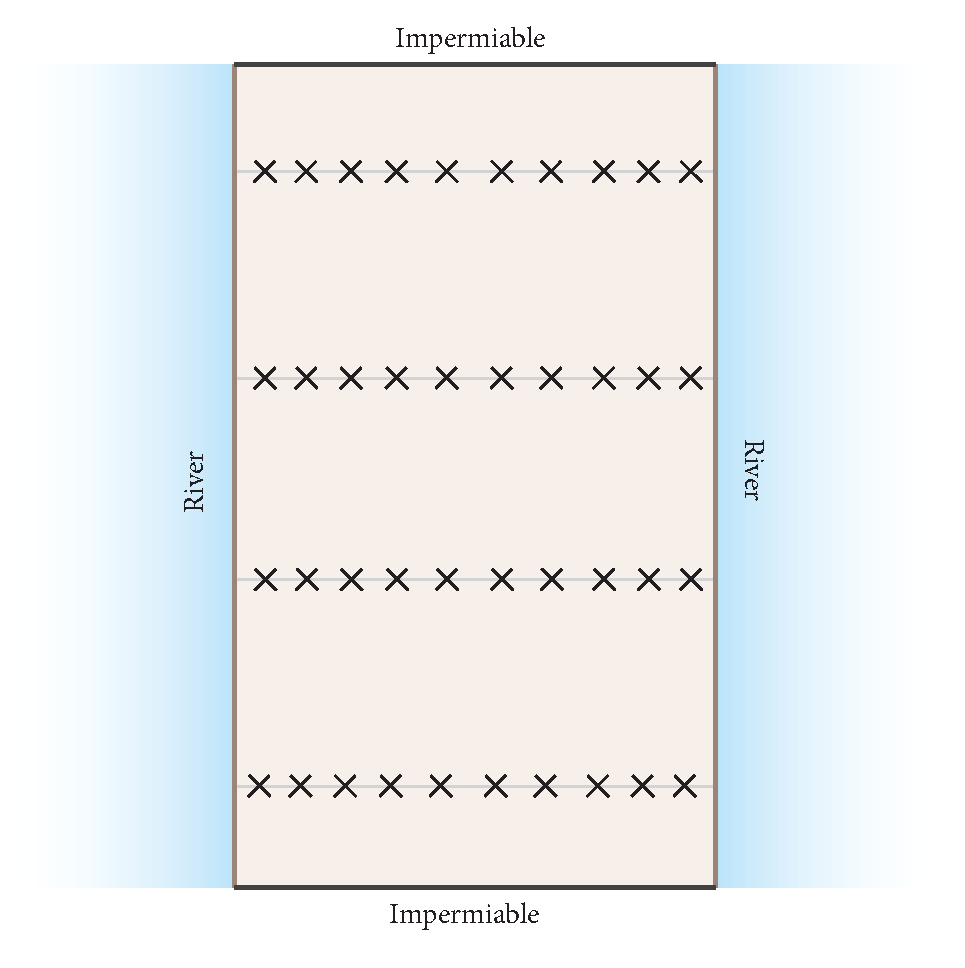
\includegraphics[width=.7\textwidth]{figs/site.pdf} 
   \caption{Study area, x's represent pumping locations.  Impermiable boundaries exist on the north and south sides and rivers on the east and west sides.}
   \label{fig:flow}
\end{figure}

The City is interested in several alternatives for putting in pumps.  

A Linked Simulation Optimization (LSO) was carried out for a well-aquifer system. The simulation, originally implemented in \verb"Fortran 77", was rewritten in \verb"Matlab".  The optimization was also carried out in \verb"Matlab" using the \verb"fmincon" function. 


\section*{Simulation Model}
The steady state simulation model has the form 
$$
T\frac{\partial^2h}{\partial x^2}+\sum_iQ_i\delta(x-x_i)=0
$$
$$0\leq x\leq L$$
$$h(0)=1,\,\,\,\,\,h(L)=1$$
where $T$ is the transmissivity, $h$ is the head, the $Q_i$'s are pumping rates and $\delta(\cdot)$ is the Dirac delta function. The given boundary conditions are implicitly constant in time. The parameter values are
\begin{center}
\begin{tabular}{cc}
\toprule
Parameter & Value\\
\midrule
T & 1 m$^2$/day\\
L & 1 m\\
\bottomrule
\end{tabular}
\end{center}
Though the transmissivity has no effect on the final solution.

Using a central difference approximation for the spatial derivative at $n$ internal leads to a system of $n$ algebraic equations. Since we have no temporal derivatives, the system can be written in the form 
$$
A\mathbf{h}+\mathbf{f}=0
$$
where A is a tridiagonal matrix, $\mathbf{h}$ is the nodal values of head, and $\mathbf{f}$ is  a vector with information about the boundary conditions and pumping at each node.  Using this notation, the nodal values of head are given by 
$$
\mathbf{h}=-A^{\mbox{-}1}\mathbf{f}.
$$
The nodal values of head are computed in the function \verb"zack", given in the source code section.  The function \verb"zack" takes in the pumping rates at each of the internal nodes and passes back head values.  The call statement is
\begin{center}
\texttt{h=zack(Q)}.
\end{center}



\section*{Optimization Model}
As per the LSO approach the simulation model was used to determine optimal pumping rates and well placement given certain constraints.  The optimization problem is 
$$\mbox{max}\,\,z=\sum_{i=1}^nh_i$$
%?? 
subject to: 
$$\sum_iQ_i\geq D $$
$$h_i \geq h^* \,\,\,\forall i $$
$$Q_i\geq 0 \,\,\, \forall i.$$

Where D is the demand which is to be determined.  The parameters values here are 
\begin{center}
\begin{tabular}{cc}
\toprule
Parameter & Value\\
\midrule
$h^*$ & .7 m\\
$n$ & 10 \\
\bottomrule
\end{tabular}
\end{center}


\section*{Implementation}
As alluded to in the introduction the optimization was carried out in \verb"Matlab" with the function \verb"fmincon" which is a general purpose function for constrained nonlinear minimization.  The above maximization was made into the minimization of the negative head values.  The calling procedure is very similar to \texttt{Minos} in that two auxiliary functions are needed to evaluate the constraints and the objective function.  Each auxiliary function calls the simulation model when necessary.  A schematic representation of the calling structure is shown in in Figure 1.  Source code is given in the source code section.

\begin{figure}[!h] %  figure placement: here, top, bottom, or page
   \centering
   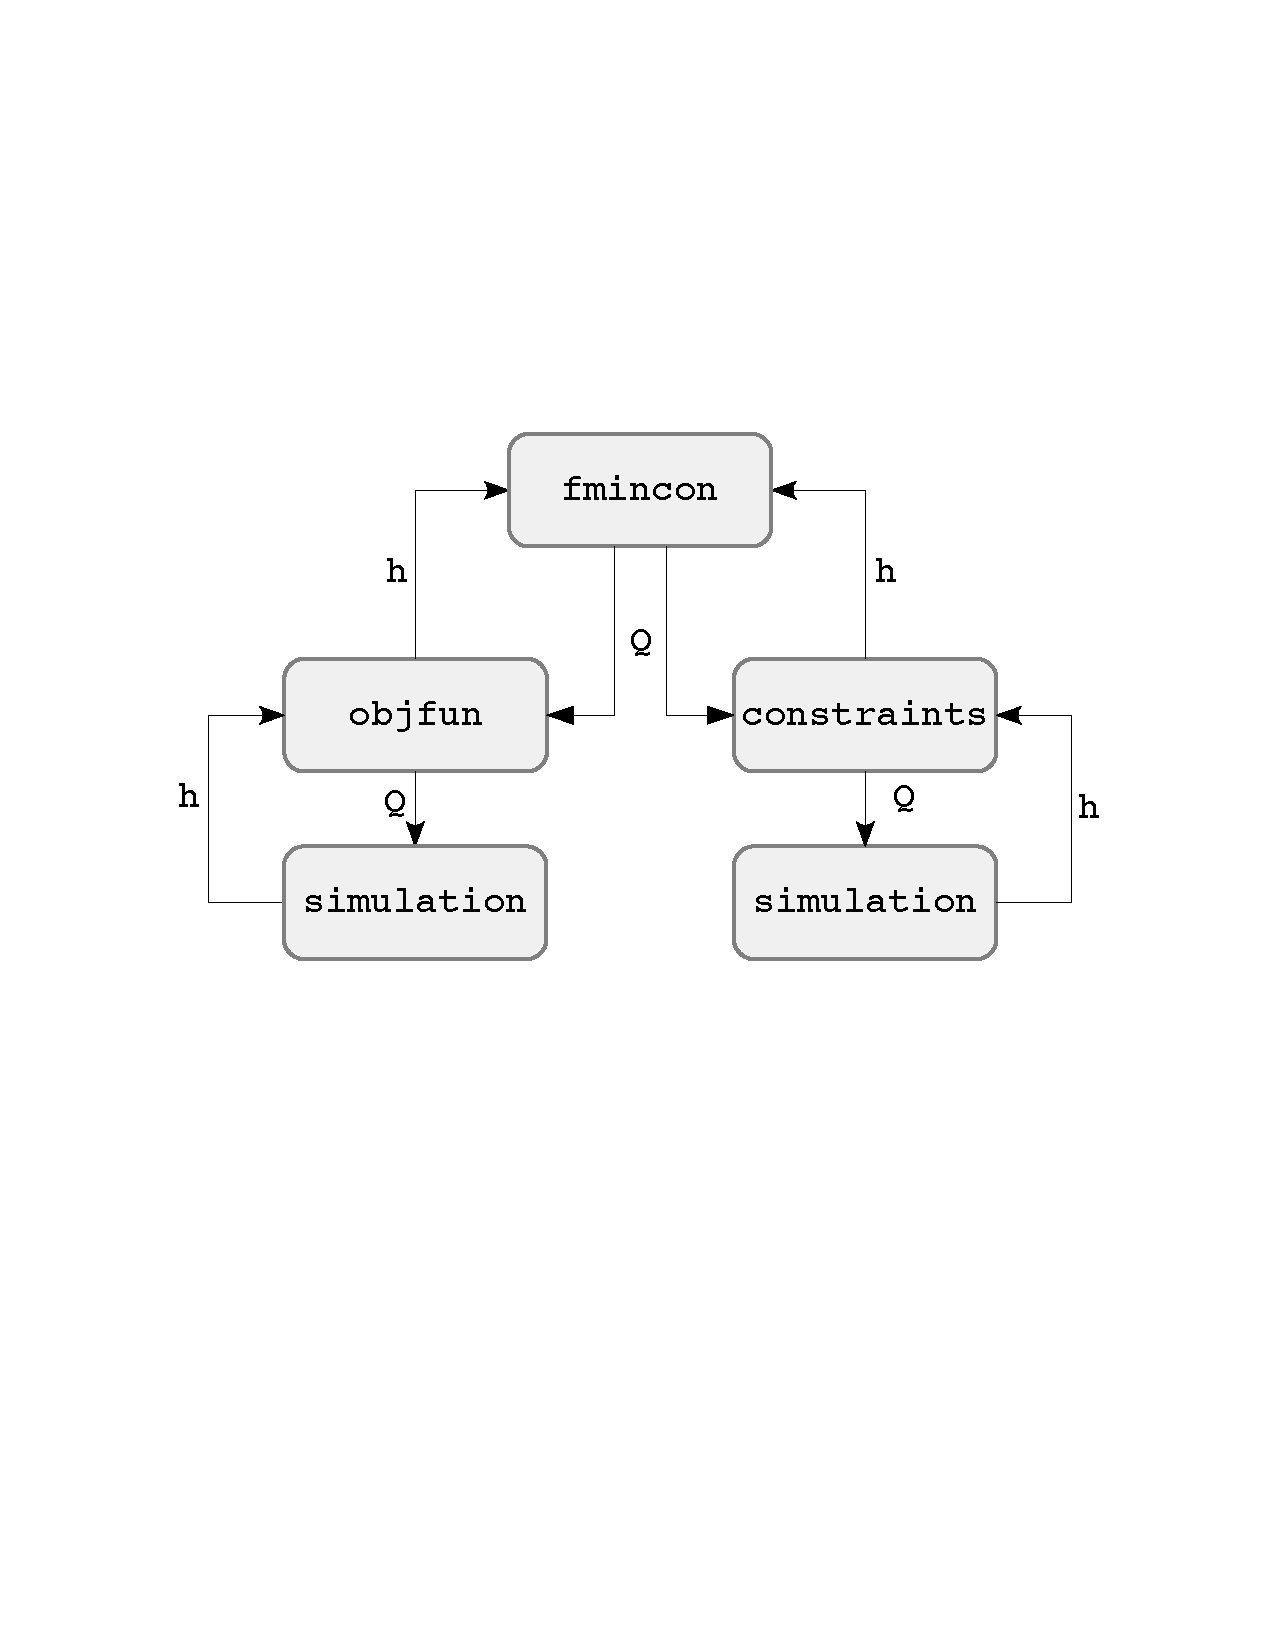
\includegraphics[width=4in]{figs/flow.pdf} 
   \caption{Schematic representation of the optimization procedure in \texttt{Matlab}.}
   \label{fig:flow}
\end{figure}

\newpage
\section*{Results}

The maximum demand that was able to be fulfilled without violating the head constraint was $D^*$=6.6 m$^3$/day. As long as the demand was less than $D^*$ then the optimization split the demand in half and placing $D^*/2$ at both node 1 and node 10.  The head profile when $D^*$=6.6 is shown in figure 2.  

A plot of the objective function $z$ versus the demand is shown in Figure 3.  Sample output from \verb"fmincon" is provided in the sample output section.



\begin{figure}[!h] %  figure placement: here, top, bottom, or page
   \centering
   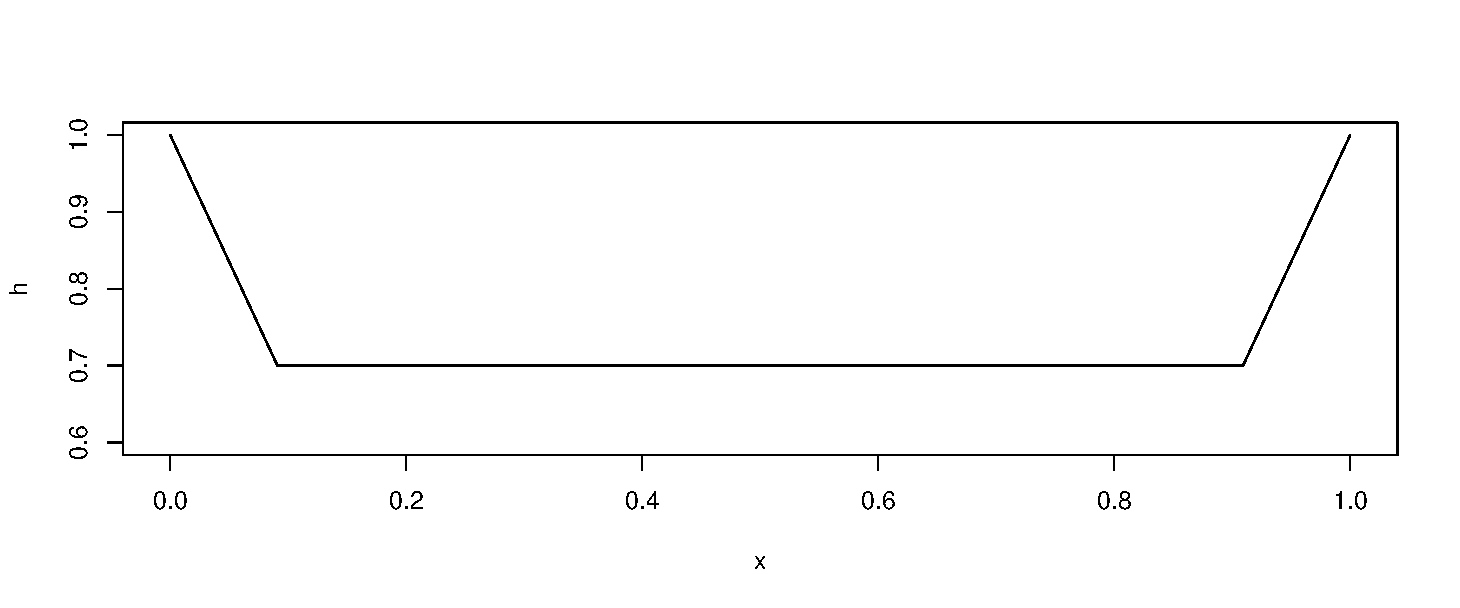
\includegraphics[width=\textwidth]{figs/head.pdf} 
   \caption{head profile when $D^*$=6.6 m$^3$/day.}
   \label{fig:head}
\end{figure}

\begin{figure}[!h] %  figure placement: here, top, bottom, or page
   \centering
   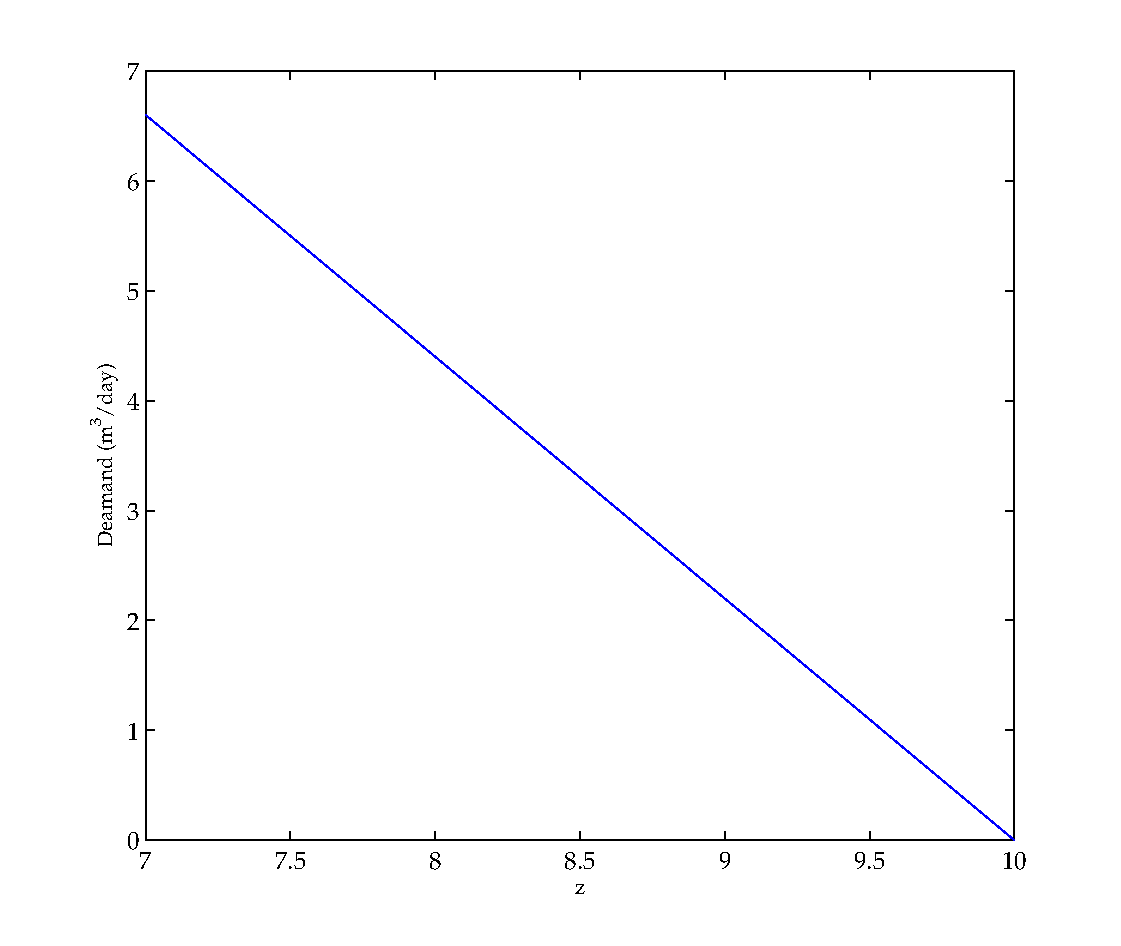
\includegraphics[width=6in]{figs/zvd} 
   \caption{The objective function ($\sum h$) versus the Demand.}
   \label{fig:zvd}
\end{figure}

\clearpage
\section{Source Code and Sample output}
\small
\subsection{Main Program}
\begin{verbatim}
%this mfile sets up the runs the optimiztion
%           max f = sum(h_i)     maximize gw head
%   subject to:
%           sum(Q_i) = D         pumping must satisfy demand
%           h_i >= h*            head levels must not drop below standard
%           Q_i >= 0             no injection 
%the three auxilary files are:
%   objfun.m -      z = objfun(Q) 
%                   evaluates the objective function given the Q_i's (by
%                   calling zack)
%   zack.m -        h=zack(Q)
%                   solves the diffusion equation, takes pumping rates, gives
%                   back heads
%   constraints.m - evaluates the nonlinear constraints (calls zack)
%


options = optimset('LargeScale','off');
x0=[1 0 0 0 1 0 0 0 0 1];

diary('op.out')
[x,fval,exitflag,output] = fmincon(@objfun,x0,[],[],[],[],[],[],@constraints,options);

if(exitflag)
    'All that stuff up there means OPTIMAL SOLUTION FOUND!!!!'
    'The pumping rate was:'
    6.5
    'The minimum head level was:'
    0.7
    'The optimal pumping rates:'
    q=x;
    q
    h=zack(-x,10);
    'The head levels at optimallity:'
    h'
    'output saved to op.out'
end
diary off
\end{verbatim}
\clearpage
\subsection{Objective Function}
\begin{verbatim}
function f = objfun(x)
    %this function evaluates the objective function

    
    n=10;    %number of nodes
    
    %x is the pumping rates, must be negative for the model
    h=zack(-x,n);
    
    %fmincon minimizes by default so f must be negative to maximize
    f=-sum(h);
\end{verbatim}
\subsection{Constraints}
\begin{verbatim}
function [c, ceq] = constraints(x)
  % This function evaluates the constraints 
  
  n=10;
  h=zack(-x,n);
  dem=6.6;
  minh=.7;      %h*, the minimum head value
  
  
  %the first part is the nonlinear min head constraint
  %the second part is the nonnegativity pumping constraint
  c = [ (minh-h)', -x ] ; 
  
  % The demand constraint rearranged to make leq
  % Not really a nonlinear constraint but easier to put here
  ceq = dem-sum(x); %dem-sum(x);
\end{verbatim}
\newpage
\subsection{Simulation Model}
\begin{verbatim}
function h=zack(q,n)
    %solves the diffusion equation given pumping rates q
    %  n is the number of internal nodes

      dx=1/(n+1);   %distance between nodes
      d=1;          %transmissivity
      xl=1;         %right boundary condition
      xr=1;         %left boundary condition

      a=zeros(n,n);
      b=zeros(n,1);
      
      b(1)=d*xl/(dx^2);
      b(n)=d*xr/(dx^2);

      for  i=1:n
          b(i)=b(i)+q(i)/dx;
      end 

      for  i=1:n
          a(i,i)=d*(+2./(dx^2));
          if (i~=n)
              a(i,i+1)=-d/(dx^2);
          end
          if(i~=1)
              a(i,i-1)=-d/(dx^2);
          end
      end
      
      h=a\b;
\end{verbatim}
\subsection{Sample Output}
\begin{verbatim}
Optimization terminated: magnitude of search direction less than 2*options.TolX
 and maximum constraint violation is less than options.TolCon.
Active inequalities (to within options.TolCon = 1e-06):
  lower      upper     ineqlin   ineqnonlin
                                     1
                                     2
                                     3
                                     4
                                     5
                                     6
                                     7
                                     8
                                     9
                                    10
                                    12
                                    13
                                    14
                                    15
                                    16
                                    17
                                    18
                                    19
The pumping rate was:
    6.6000
The minimum head level was:
    0.7000
The optimal pumping rates:
    3.3000
   -0.0000
   -0.0000
   -0.0000
   -0.0000
   -0.0000
   -0.0000
   -0.0000
   -0.0000
    3.3000
The head levels at optimallity:
h =
    0.7000
    0.7000
    0.7000
    0.7000
    0.7000
    0.7000
    0.7000
    0.7000
    0.7000
    0.7000
output saved to op.out
\end{verbatim}


\end{document}  